\chapter{Hardware \& Programmiermöglichkeiten}
\label{ch:hardprog}
In diesem Kapitel soll die für die mobilen Einheiten verwendete Hardware und ihre Programmiermöglichkeiten näher beleuchtet werden.
Als mobile Einheiten werden in dieser Arbeit hauptsächlich Tags behandelt: Tags sind kleine Geräte, die ausschließlich zur Ortung und damit einhergehender Identifikation genutzt werden.\\
Diese Arbeit behandelt jedoch ebenfalls die Ortung mittels Smartphones mit dem Android Betriebssystem von Google \cite{google2017android}, um diese in das System einzugliedern und bei Personen, die ein Firmenhandy besitzen die Notwendigkeit eines zusätzlichen Tags zu eliminieren.\\
Ein Smartphone kann auch ohne Software für die Ortung nicht die geforderten 6 Monate Batterielaufzeit erfüllen, derartige Anforderungen werden deshalb fallen gelassen. 
Stattdessen muss ein Smartphone mindestens eine 12-stündige Schicht ohne Ladevorgang auskommen, da sonst ein Bereichswechsel nicht mehr erkannt werden kann.
Lösungen mit geringem Energieverbrauch werden dennoch bevorzugt.

\begin{figure}[h]
  \centering
	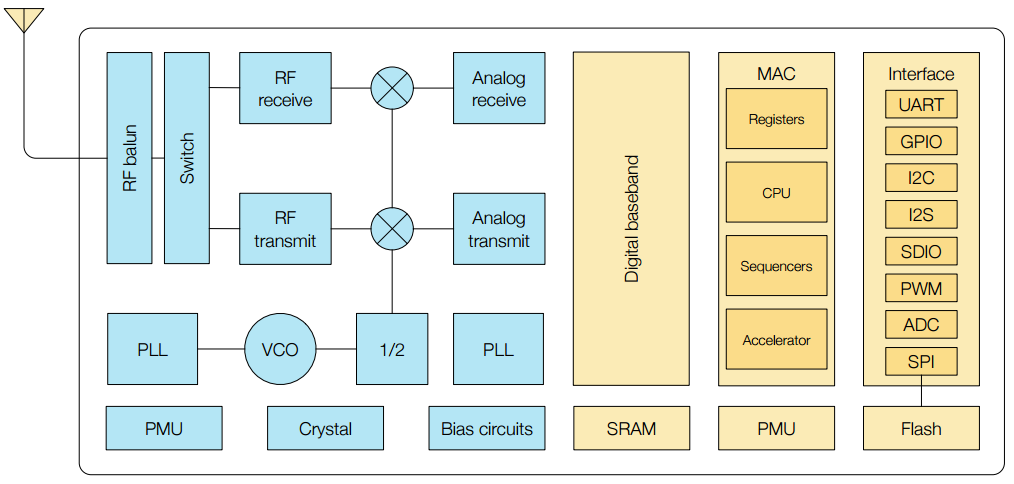
\includegraphics[width=\textwidth]{images/espblock.png}
  \caption{Blockdiagramm des ESP8266, aus \cite{espressif2017esp8266}}
  \label{fig:espblock}
\end{figure}

\section{ESP8266}
Für WLAN-basierte Tags kommt der ESP8266 von Espressif in den Modulen ESP12-S beziehungsweise ESP12-F zum Einsatz.
Der ESP8266 zeichnet sich durch einen niedrigen Energieverbrauch und viele Freiheiten bei der Programmierung aus, die Module ESP12-S und ESP 12-F unterscheiden sich dabei hauptsächlich durch ihre Antenne, siehe Abb. \ref{fig:espmodules}.
Das neuere ESP12-F sollte eine höhere Reichweite entfalten, dies wird noch Gegenstand eines Experiments sein.\\
Der Esp8266 besitzt neben einer CPU eine 802.11b/g/n/e/i-fähige WLAN-Einheit und diverse andere, kabelgebundene Kommunikationsstandards wie zum Beispiel GPIO, I2C und SPI, siehe Abb. \ref{fig:espblock}.
Der Chip selbst besitzt weder einen Flashspeicher für Programme und Daten noch eine Antenne, diese werden auf dem Modul, z.B. ESP-12F, integriert \cite{espressif2017esp8266}.
Espressif gibt im Datenblatt auch Aufschluss über den Energieverbrauch des Chips, siehe dazu Abb. \ref{fig:esppower}.




\begin{figure}[h]
  \centering
	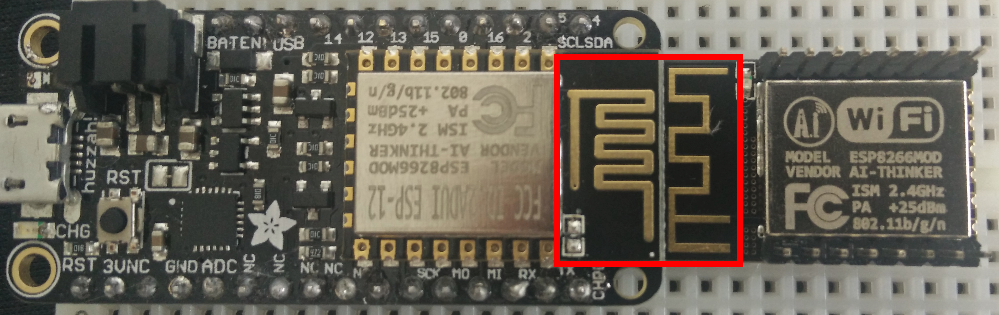
\includegraphics[width=\textwidth]{images/espmodules.png}
  \caption{Vergleich der Antennen, links: ESP12-S verbaut auf einem Adafruit Feather Huzzah, rechts: ESP12-F}
  \label{fig:espmodules}
\end{figure}

\begin{figure}[h]
  \centering
	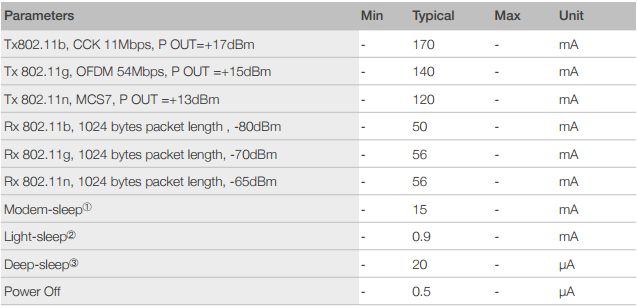
\includegraphics[width=\textwidth]{images/esppower.png}
  \caption{Energieverbrauch des ESP8266 bei verschiedenen Operationen, aus \cite{espressif2017esp8266}}
  \label{fig:esppower}
\end{figure}

\section{Texas Instruments SensorTag}
Für das Bluetooth-basierte Tag wird das SensorTag von Texas Instruments verwendet.
